\documentclass[11pt]{article}
\usepackage{tikz}

\makeatletter
\pgfkeys{
  /pgf/lh/.initial=30  % Default angle is 30 degrees
}

% Declare meaningful coordinate registers
\newdimen\my@N  % North (top) y coordinate
\newdimen\my@E  % East (right) x coordinate
\newdimen\my@W  % West (left) x coordinate
\newdimen\my@S  % South (bottom) y coordinate
\newdimen\my@Cx % Center x coordinate
\newdimen\my@Cy % Center y coordinate

% Other useful registers
\newdimen\my@halfwidth
\newdimen\my@halfheight
\newdimen\my@offset

% Macro to set NESW coordinates from southwest/northeast
\def\setmy@NEWSC{%
  \southwest
  \my@W=\pgf@x%
  \my@S=\pgf@y%
  \northeast
  \my@E=\pgf@x%
  \my@N=\pgf@y%
  % Calculate center
  \my@Cx=.5\my@W%
  \advance\my@Cx by.5\my@E%
  \my@Cy=.5\my@S%
  \advance\my@Cy by.5\my@N%
  % Calculate half dimensions
  \my@halfwidth=\my@E%
  \advance\my@halfwidth by-\my@W%
  \my@halfwidth=.5\my@halfwidth%
  \my@halfheight=\my@N%
  \advance\my@halfheight by-\my@S%
  \my@halfheight=.5\my@halfheight%
}

\pgfdeclareshape{lh}{
  % Inherit anchors from rectangle
  \inheritsavedanchors[from=rectangle]
  \inheritanchor[from=rectangle]{center}
  \inheritanchor[from=rectangle]{north}
  \inheritanchor[from=rectangle]{south}
  \inheritanchor[from=rectangle]{east}
  \inheritanchor[from=rectangle]{west}
  \inheritanchor[from=rectangle]{north east}
  \inheritanchor[from=rectangle]{north west}
  \inheritanchor[from=rectangle]{south east}
  \inheritanchor[from=rectangle]{south west}
  
  % Saved anchor for inner north west
  \savedanchor\innernorthwest{%
    % Get text box dimensions
    \pgf@x=.5\wd\pgfnodeparttextbox%
    \pgf@y=.5\ht\pgfnodeparttextbox%
    \advance\pgf@y by.5\dp\pgfnodeparttextbox%
    % Add inner sep
    \pgfmathsetlength\my@halfwidth{\pgfkeysvalueof{/pgf/inner xsep}}%
    \pgfmathsetlength\my@halfheight{\pgfkeysvalueof{/pgf/inner ysep}}%
    \advance\pgf@x by\my@halfwidth%
    \advance\pgf@y by\my@halfheight%
    % Check minimum dimensions
    \pgfmathsetlength\my@halfwidth{\pgfkeysvalueof{/pgf/minimum width}}%
    \pgfmathsetlength\my@halfheight{\pgfkeysvalueof{/pgf/minimum height}}%
    \ifdim\pgf@x<.5\my@halfwidth\pgf@x=.5\my@halfwidth\fi%
    \ifdim\pgf@y<.5\my@halfheight\pgf@y=.5\my@halfheight\fi%
    % Store half dimensions
    \my@halfwidth=\pgf@x%
    \my@halfheight=\pgf@y%
    % Calculate offset
    \pgfmathsetmacro{\hexangle}{\pgfkeysvalueof{/pgf/lh}}%
    \show\hexangle
    \pgfmathsetlength\my@offset{\my@halfheight*tan(\hexangle)}%
    \showthe\my@offset
    % Set final position (inner north west)
    \pgf@x=-\my@halfwidth%
    \advance\pgf@x by\my@offset%
    \pgf@y=\my@halfheight%
  }
  
  % Inner anchors - COMMENTED OUT FOR TESTING
  % \anchor{inner-north-west}{\innernorthwest}
  % \anchor{inner-north-east}{\innernorthwest\pgf@x=-\pgf@x}
  % \anchor{inner-south-west}{\innernorthwest\pgf@y=-\pgf@y}
  % \anchor{inner-south-east}{\innernorthwest\pgf@x=-\pgf@x\pgf@y=-\pgf@y}
  
  % Background path
  \backgroundpath{%
    % Get NESW coordinates
    \setmy@NEWSC
    % Get angle and calculate offset
    \pgfmathsetmacro{\hexangle}{\pgfkeysvalueof{/pgf/lh}}%
    \pgfmathsetlength\my@offset{\my@halfheight*tan(\hexangle)}%
    \showthe\my@offset
    % Draw hexagon using meaningful coordinates
    \pgfpathmoveto{\pgfpoint{\my@W}{\my@Cy}}% west vertex
    \pgfpathlineto{\pgfpoint{\my@W+\my@offset}{\my@N}}% inner NW
    \pgfpathlineto{\pgfpoint{\my@E-\my@offset}{\my@N}}% inner NE
    \pgfpathlineto{\pgfpoint{\my@E}{\my@Cy}}% east vertex
    \pgfpathlineto{\pgfpoint{\my@E-\my@offset}{\my@S}}% inner SE
    \pgfpathlineto{\pgfpoint{\my@W+\my@offset}{\my@S}}% inner SW
    \pgfpathclose%
  }
}
\makeatother

\begin{document}

% Test the lh shape with default angle (30 degrees)
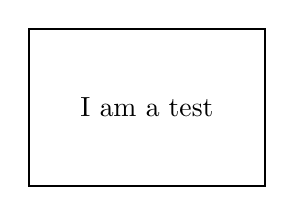
\begin{tikzpicture}
  \node[lh, draw, thick, minimum width=3cm, minimum height=2cm] (hex) at (0,0) {I am a test};
  % Debug: drop a red circle on inner north west anchor - COMMENTED OUT
  % \fill[red] (hex.inner-north-west) circle (2pt);
\end{tikzpicture}

\vspace{1cm}

% Test with different angles
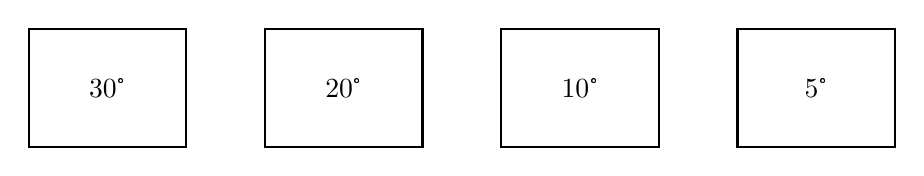
\begin{tikzpicture}
  \node[lh, draw, thick, lh=30, minimum width=2cm, minimum height=1.5cm] (hex1) at (0,0) {30°};
  % \fill[red] (hex1.inner-north-west) circle (2pt);
  
  \node[lh, draw, thick, lh=20, minimum width=2cm, minimum height=1.5cm] (hex2) at (3,0) {20°};
  % \fill[red] (hex2.inner-north-west) circle (2pt);
  
  \node[lh, draw, thick, lh=10, minimum width=2cm, minimum height=1.5cm] (hex3) at (6,0) {10°};
  % \fill[red] (hex3.inner-north-west) circle (2pt);
  
  \node[lh, draw, thick, lh=5, minimum width=2cm, minimum height=1.5cm] (hex4) at (9,0) {5°};
  % \fill[red] (hex4.inner-north-west) circle (2pt);
\end{tikzpicture}

\vspace{1cm}

% Test with different styling and show all inner anchors
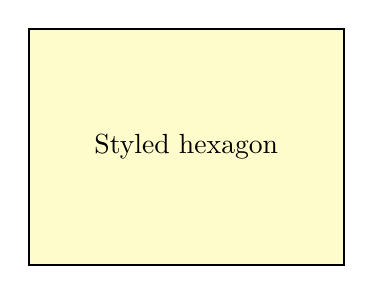
\begin{tikzpicture}
  \node[lh, draw, thick, fill=yellow!20, lh=25, minimum width=4cm, minimum height=3cm] (hex) at (0,0) {Styled hexagon};
  % Show all inner anchors - COMMENTED OUT
  % \fill[red] (hex.inner-north-west) circle (2pt) node[above left, font=\tiny] {inner NW};
  % \fill[blue] (hex.inner-north-east) circle (2pt) node[above right, font=\tiny] {inner NE};
  % \fill[green] (hex.inner-south-west) circle (2pt) node[below left, font=\tiny] {inner SW};
  % \fill[orange] (hex.inner-south-east) circle (2pt) node[below right, font=\tiny] {inner SE};
\end{tikzpicture}

\end{document}
